A topologia sempre foi vista como uma área de abstração da matemática, sem
espaço para aplicações. Ela é usada para o estudo de diversos espaços
em sua forma abstrata, auxiliando matemáticos em diversas demonstrações
de teoremas e dando uma base fundamental para grande parte da teoria matemática
usada no dia a dia~\cite{Poincare1895}.

Certas propriedades dos espaços topológicos são estudadas através da
topologia algébrica, dando algumas informações, como o número de componentes
conexas por caminhos de um espaço e buracos. A princípio esta é uma área altamente
abstrata da matemática,  nos últimos anos esta visão foi mudando,
com o desenvolvimento da Homologia Persistente e Análise Topológica de Dados.

Um conjunto de dados, geralmente um subconjunto finito de algum espaço métrico,
pode ser estudado através da homologia persistente e assim obtemos informações
topológicas do objeto em estudo.

O pipeline da análise topológica de dados pode ser divido nos seguintes passos:
\begin{itemize}
  \item A entrada do algoritmo pode ser um conjunto de pontos ou alguma matriz
  de distância/similaridade do conjunto de dados.
  \item A construção de um objeto combinatorial em cima do conjunto de dados ou
  da matriz de distância. Geralmente uma filtração ou um complexo simplicial.
  \item A partir da filtração ou do complexo simplicial é possível extrair informações
  topológicas e geométricas do conjunto de dados, por exemplo o número de
  componentes conexas, como um algoritmo de Clustering.
  \item Por fim a interpretação dos dados obtidos e possível pós processamento
  para a utilização em outros algoritmos, como os de classificação ou regressão.
\end{itemize}

Neste capítulo descrevemos de forma ingênua a homologia persistente, começando com
filtrações, passando pelos espaços vetoriais associados
aos complexos simpliciais e chegando ao algoritmo de homologia persistente.
Mostraremos também como interpretar os resultados obtidos.
A \autoref{fig:pipeline_hp} mostra os passos para utilizar esta ferramenta em um conjunto de dados.

\begin{figure}
  \centering
  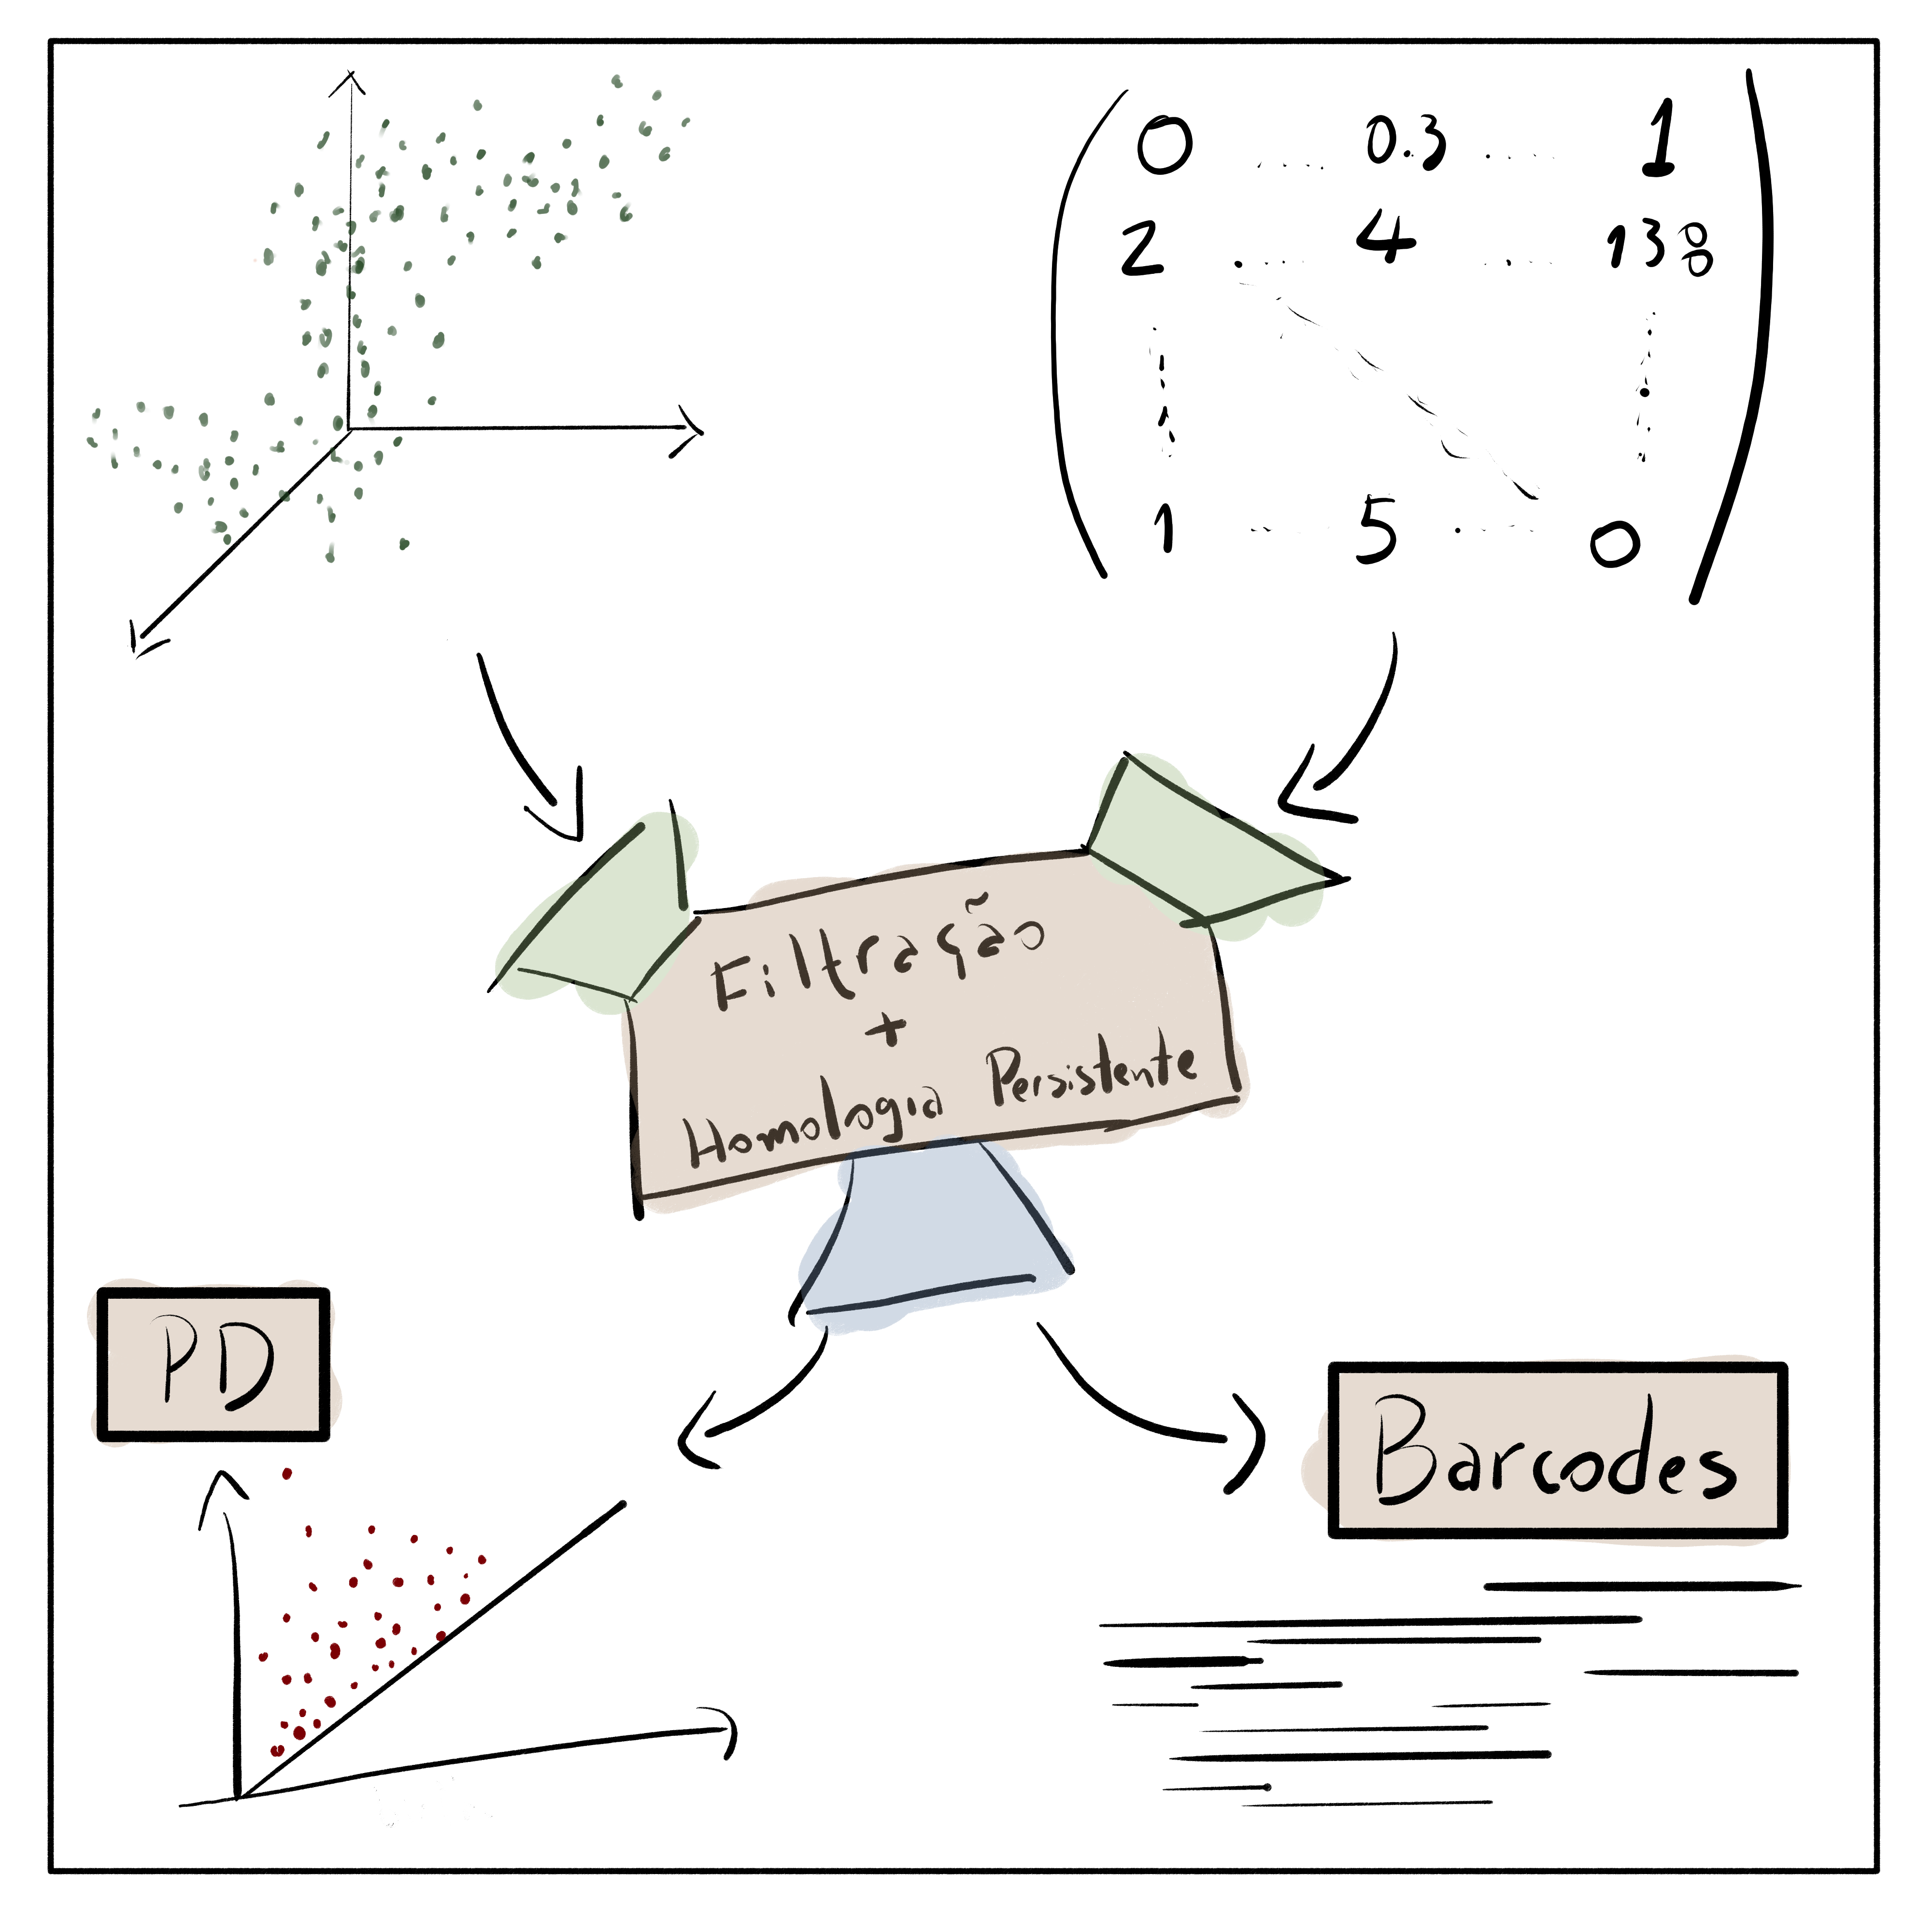
\includegraphics[width=0.7\textwidth]{images/pipeline_hp.png}
  \caption{Representação do pipeline para a utilização da homologia persistente
          com um conjunto de dados.}
  \label{fig:pipeline_hp}
\end{figure}


\section{Filtrações}
A filtração de um conjunto de dados é o primeiro passo na nossa sequência apresentada
na \autoref{fig:pipeline_hp}.
Dado um conjunto de dados precisamos construir um objeto combinatorial de forma
que possa ser analisado do ponto de vista da topologia assim como computacionalmente.
A filtração é este objeto que captura as mudanças do conjunto dada uma escala.

Algumas definições se fazem necessárias para entendermos o que é a filtração
e qual o seu papel na análise topológica de dados. Começamos definindo um simplexo,
primeiro objeto combinatorial que é a base da filtração.

\begin{defi}
  Sejam $v_0, v_1, \dots, v_k \in \mathbb{R}^n$ linearmente afins, ou seja $\{v_1 - v_0, \dots, v_k - v_0\}$
  é um conjunto linearmente independente. O $k$-simplexo definido pelos pontos acima,
  chamados de vértices, é a envoltória convexa, definida na~\autoref{eq:envconv}.
  \begin{equation}
    \label{eq:envconv}
    \Set{\sum_{i=0}^k \lambda_i v_i \ | \ \sum_{i=0}^k \lambda_i = 1 \text{ e }
          \lambda_i \ge 0, \ \forall i}.
  \end{equation}
  Denotamos o $k$-simplexo por $<v_0, \dots, v_k>$.
\end{defi}

Note que para $k = 0$, temos um único vértice. Para $k=1$, temos uma reta, já
para $k=2$ temos um triângulo preenchido. E no caso $k=3$, um tetraedro. Os
simplexos podem ser vistos na~\autoref{fig:ksimpl}. Além disso, dizemos que a dimensão
do $k$-simplexo é $k$. A envoltória convexa de qualquer subconjunto dos vértices
de um simplexo $\sigma$ é chamado de face de $\sigma$.

\begin{figure}
  \centering
  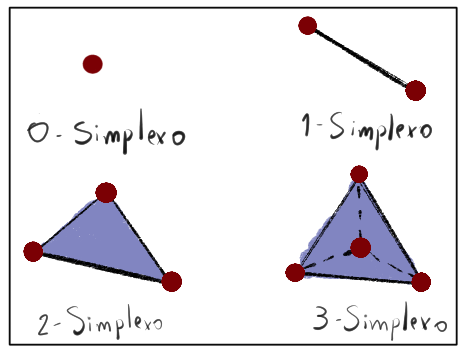
\includegraphics[width=0.7\textwidth]{images/ksimpl.png}
  \caption{Exemplos de $k$-simplexos para $k \in \Set{0,1,2,3}$.}
  \label{fig:ksimpl}
\end{figure}

Tendo definido os $k$-simplexos, podemos definir o complexo simplicial.
\begin{defi}
    Um complexo simplicial $K$ é uma coleção de simplexos satisfazendo as seguintes
    relações:
    \begin{itemize}
      \item Dado $\sigma \in K$, temos que para toda face $\tau \subset \sigma$
            vale $\tau \in K$.
      \item A interseção de dois simplexos é face de ambos os simplexos, em outras palavras,
      $\sigma, \tau \in K$ implica que $\sigma \cap \tau \subset \sigma$ e
      $\sigma \cap \tau \subset \tau$.
    \end{itemize}
\end{defi}
A segunda condição é necessária para evitar casos patológicos como mostrado na
\autoref{fig:simp_path}. Dizemos que a dimensão do complexo simplicial $K$ é a maior dimensão dentre os
simplexos em $K$. Podemos definir agora a filtração de um complexo simplicial.
\begin{figure}
  \centering
  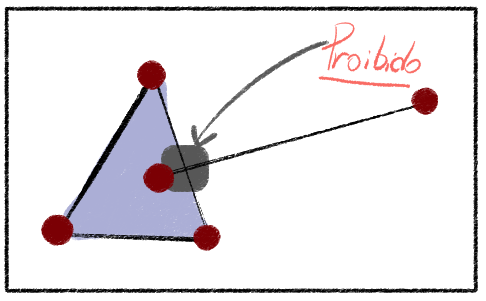
\includegraphics[width=0.7\textwidth]{images/simp_path.png}
  \caption{Exemplo em que a interseção de dois simplexos não é um simplexo.}
  \label{fig:simp_path}
\end{figure}
\begin{defi}
  Seja $K$ um complexo simplicial. Definimos uma filtração de $K$ sendo uma
  sequência de subconjuntos $K_i \subset K$, com $i \in \{ 1, \dots, n \}$,
  de tal forma que $K_i$ é um complexo simplicial para todo $i$ e vale que
  \begin{equation*}
    K_1 \subset \dots \subset K_{n-1} \subset K_n = K.
  \end{equation*}
\end{defi}
Na~\autoref{fig:filtracao_exemplo} temos um exemplo de filtração para um complexo
simplicial.

\begin{figure}[hbt]
  \centering
  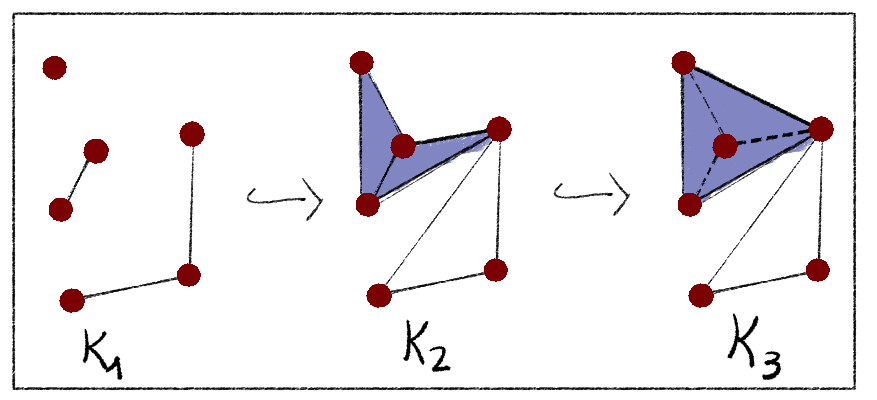
\includegraphics[width=0.7\textwidth]{images/filtracao_exemplo.png}
  \caption{Exemplo de filtração para um complexo simplicial $K$.}
  \label{fig:filtracao_exemplo}
\end{figure}


\subsection{Complexo de \v{C}ech}
Para construir complexos simpliciais a partir dos dados, precisamos abstrair
a noção de um simplexo simplicial. Na definição dada anteriormente, temos uma
representação geométrica do que é um simplexo, mas podemos abstrair tal noção
dando origem aos \textit{complexos simpliciais abstratos}.
\begin{defi}
  Seja $X$ um conjunto finito com pontos quaisquer. Seja $F$ um conjunto de
  subconjuntos não-vazios de $X$. Dizemos que $F$ é um complexo simplicial abstrato de
  $X$ se a seguinte condição é satisfeita.
  \begin{itemize}
    \item Se para todo $\sigma \in F$, temos que para todo subconjunto
          $\sigma' \subset \sigma$ está em $F$ também.
  \end{itemize}
  Cada elemento $\sigma \in F$ é chamado de simplexo.
\end{defi}

\begin{ex}
  Seja $X=\Set{a,b,c}$ e considere $F=\Set{\lp a \rp, \lp b \rp, \lp c \rp,
  \lp a,b \rp, \lp a,c \rp, \lp b,c \rp}$. Precisamos mostrar que F é um complexo
  simplicial abstrato. Seja $\sigma=\Set{a,c}$. Note que seus subconjuntos são
  $\Set{a}$ e $\Set{c}$, além disso ambos pertencem a $F$. De forma análoga, mostramos
  que para qualquer outro simplexo, suas faces (subconjuntos) estão em $F$.
\end{ex}
Podemos realizar os complexos simpliciais abstratos geometricamente, ou seja,
apesar de trabalharmos com conjuntos de elementos quaiser, podemos incluir
esses complexos em algum $\mathbb{R}^n$ e assim visualiza-los. Para obtermos
o complexo simplicial \textit{geométrico}, associamos a cada simplexo abstrato $\sigma$
um simplexo geométrico. Por exemplo, se adotarmos o complexo simplicial abstrato
$F$ acima mostrado, teriamos que sua realização geométrica seria um triângulo
sem preenchimento, como é mostrado na~\autoref{fig:abs_real}.

\begin{figure}
  \centering
  
\includegraphics[width=0.7\textwidth]{images/placeholder.png}
  \caption{Exemplo de um complexo simplicial abstrato e sua realização geométrica}
  \label{fig:abs_real}
\end{figure}
Observe que se o nosso conjunto $X$ for um subconjunto finito de $\mathbb{R}^d$,
podemos ter simplexos de dimensão maiores do que $d$, ou seja, não podem ser
realizados (ou visualizados) em $\mathbb{R}^d$ necessariamente. Um exemplo dessa
situação pode ser visto na~\autoref{fig:abs_nonembed} com o conjunto
$X=\Set{x_1, x_2, \dots, x_n} \subset \mathbb{R}^2$ e $n>3$.

\begin{figure}
  \centering
  
\includegraphics[width=0.7\textwidth]{images/placeholder.png}
  \caption{Cada ponto na imagem corresponde a realização geométrica dos pontos
  de X. Note que temos um tetraedro neste caso, apesar de estarmos com pontos em
  $\mathbb{R}^2$.}
  \label{fig:abs_nonembed}
\end{figure}
Essa é uma grande diferença entre os complexos simpliciais geométricos e abstratos.
Uma vez tendo definido os complexos simpliciais abstratos, podemos definir o
\textit{complexo de \v{C}ech}.

\begin{defi}
  Seja $X$ um conjunto de pontos $\Set{x_1, \dots, x_n}$ em $\mathbb{R}^d$. O complexo
  de \v{C}ech de X para um valor real $r>0$ é o conjunto $C^r(X)$, onde
  $\sigma = <x_{i_1}, \dots, x_{i_k}> \in C^r(X)$ se, e somente se vale a seguinte
  condição
  \begin{equation*}
    \bigcap_{j=1}^k B(x_{i_j},r) \neq \emptyset.
  \end{equation*}
\end{defi}
A definição acima nos diz que quando temos $k$ pontos cujas bolas de raio $r$
centradas neles se intersectam, adicionamos um $k$ simplexo no complexo simplicial
abstrato, o que seria apenas o conjunto desses pontos. Geometricamente falando,
se duas bolas se intersectam, adicionamos uma aresta. Se três bolas se intersectam,
adicionamos um triângulo preenchido, e assim por diante. Na~\autoref{fig:cech_ex}
temos um exemplo do complexo simplicial de \v{C}ech.
\begin{figure}[htb]
  \centering
  
\includegraphics[width=0.7\textwidth]{images/placeholder.png}
  \caption{Exemplo de um complexo de \v{C}ech para um raio $r$ fixado. Note que
  temos um tetraedro, apesar dos pontos estarem no plano.}
  \label{fig:cech_ex}
\end{figure}

Da mesma forma que definimos a filtração para um complexo simplicial geométrico,
o mesmo vale para o caso abstrato.

\subsection{Complexo de Vietoris-Rips}
O complexo de Vietoris-Rips possui uma construção similar ao complexo de \v{C}ech,
porém computacionalmente é um método mais barato, já que analisa apenas distância
entre pontos dois a dois.
\begin{defi}
  Seja $X$ um conjunto de pontos $\Set{x_1, \dots, x_n}$ em $\mathbb{R}^d$. O complexo
  de Vietoris-Rips de X para um valor real $r>0$ é o conjunto $C^r(X)$, onde o simplexo
  $\sigma = <x_{i_1}, \dots, x_{i_k}> \in V^r(X)$ se, e somente se vale a seguinte
  condição
  \begin{equation*}
    d(x_{i_k}, x_{i_j}) < r \ \forall j,l \in{1,\dots,k}.
  \end{equation*}
\end{defi}
A \autoref{fig:viet_ex} é um exemplo do complexo de Vietoris-Rips. Uma das diferenças
que a construção dos dois complexos já definidos nos dá é que no caso do complexo
de \v{C}ech temos triângulos preenchidos, e isso não ocorre para Vietoris-Rips.
\begin{figure}
  \centering
  
\includegraphics{images/placeholder.png}
  \caption{Exemplo do complexo de Vietoris-Rips com os mesmos pontos utilizados
  para a construção na \autoref{fig:cech_ex}.}
  \label{fig:viet_ex}
\end{figure}

Mesmo com as regras diferentes para a construção de complexos, temos a relação mostrada
na \autoref{eq:viet_cech}.
\begin{equation}
  C^r(X) \subset V^r(X) \subset C^{2r}(X)
\end{equation}
\subsection{Complexo \textit{Alpha Shape}}
E como uma terceira opção para a construção de um complexo simplicial através
de pontos no $\mathbb{R}^n$, temos o complexo Alpha Shape. A construção é similar
ao complexo de \v{C}ech, porém as bolas são uma interseção de bolas no $\mathbb{R}^n$
com conjuntos convexos especiais, as células de Voronoi.

O diagrama de Voronoi é um tipo especial de decomposição de um espaço métrico,
um conjunto que possui uma distância associada a ele, em especial o $\mathbb{R}^n$.
Dado um subconjunto $X \subset \mathbb{R}^n$ finito, onde $X=\Set{x_1, \dots, x_k}$,
definimos a célula de Voronoi associada ao ponto $x_i$ sendo o seguinte conjunto
\begin{equation*}
  V_i = \Set{x\in \mathbb{R}^n | d(x_i, x) \leq d(x_j, x), \ \forall j \in {1,\dots,k}},
\end{equation*}
em que $d$ é a distância euclidiana usual. 

\section{A matriz de bordo $\partial$}

\section{Redução da matriz}
